%%%%%%%%%%%%%%%%%%%%%%%%%%%%%%%%%%%%%%%%%
% Twenty Seconds Resume/CV
% LaTeX Template
% Version 1.0 (14/7/16)
%
% Original author:
% Carmine Spagnuolo (cspagnuolo@unisa.it) with major modifications by 
% Vel (vel@LaTeXTemplates.com) and Harsh (harsh.gadgil@gmail.com)
%
% License:
% The MIT License (see included LICENSE file)
%
%%%%%%%%%%%%%%%%%%%%%%%%%%%%%%%%%%%%%%%%%

%----------------------------------------------------------------------------------------
%	PACKAGES AND OTHER DOCUMENT CONFIGURATIONS
%----------------------------------------------------------------------------------------

\documentclass[letterpaper]{twentysecondcv} % a4paper for A4

% Command for printing skill overview bubbles
\newcommand\skills{ 
~
	\smartdiagram[bubble diagram]{
        \textbf{Ingeniería de}\\\textbf{Sistemas},
        \textbf{Full Stack}\\\textbf{Web Dev},
        \textbf{~~~~~OOP~~~~~~},
        \textbf{Hybrid}\\\textbf{Mobile Dev},
        \textbf{Angular}\\\textbf{4},
        \textbf{Pruebas}\\\textbf{~~Unitarias~~},
        \textbf{ORM}\\\textbf{Database}
    }
}

% Programming skill bars
\programming{{C $\textbullet$ C++  $\textbullet$ R / 3}, {Java $\textbullet$ SQL $\textbullet$ \large \LaTeX / 3.5}, {HTML5 $\textbullet$ JS $\textbullet$ Python / 5}}

% interest bars
\interest{{Desarrollo Back-End / 4}, {Desarrollo Front-End / 4.5}, {Planeación y Diagramación / 5}, {Experiencia de usuario / 5.3}}

% Projects text
\projects{
\textbf{DecAR} - An augmented reality interior decoration app for Android \\
        \textbf{CIS*6320} - An implementation of the Bicubic interpolation algorithm in C++
        \textbf{CIS*6650} - A comparative statistical study of SVM kernels, and number of hidden layers in ANN, on 5 UCI datasets
        \textbf{CIS*6660} - A data linkage project to integrate Canada's WWI casualties and 1901 Canadian census using an SVM
        \textbf{CIS*6650} - A statistical study of spurious correlations, such as correlating beer production with election outcome
}
\aboutmesidebar{
La presente es mi hoja de vida, en la cual, plasmo mi perfil académico, experiencia laboral, mis referencias personales y las competencias que considero hacen de mi perfil el indicado para desempeñarme como Desarrollador FullStack.
}
%----------------------------------------------------------------------------------------
%	 PERSONAL INFORMATION
%----------------------------------------------------------------------------------------
% If you don't need one or more of the below, just remove the content leaving the command, e.g. \cvnumberphone{}

\cvname{BRAYAN RONALDO MOJICA BARRIOS} % Your name
\cvjobtitle{ \large{Desarrollador Web \textbf{FullStack}}  } % Job
% title/career

\cvlinkedin{}
\cvgithub{ronaldomb98}
\cvfacebook{ronaldo.mojica.12}
\cvnumberphone{(+57) 311 236 6178} % Phone number
\cvphone{(8) 269 6764} % Phone number
\cvsite{} % Personal website
\cvmail{ronaldomb98@gmail.com} % Email address

%----------------------------------------------------------------------------------------

\begin{document}

%-------------------------- Personal Info ---------------------------------------
\makepersonalinfo
\begin{center}
\section{DATOS PERSONALES}
%\huge{\textbf{DATOS PERSONALES}}
\end{center}
\noindent\rule{1\textwidth}{1.4pt}

  \begin{center}
    
        \LeftBox{NOMBRES}{BRAYAN RONALDO}  \\
        \LeftBox{APELLIDOS}{MOJICA BARRIOS}       \\
        \LeftBox{FECHA DE NACIMIENTO}{MAYO 12 DE 1998}     \\
        \LeftBox{LUGAR DE NACIMIENTO}{IBAGUÉ - TOLIMA}  \\
        \LeftBox{EDAD}{19 AÑOS}  \\
        \LeftBox{CÉDULA}{1.110.590.392 DE IBAGUÉ}  \\
        \LeftBox{ESTADO CIVIL}{SOLTERO}  \\
        \LeftBox{DIRECCIÓN DE RESIDENCIA}{SMZ 5 MZ 3 CASA 16, BARRIO TUNJOS 1}  \\
        \LeftBox{TELEFONO FIJO}{2696764}  \\
        \LeftBox{CELULAR}{3112366178}  \\
        \LeftBox{CORREO ELECTRÓNICO}{ronaldomb98@gmail.com}  \\
        \LeftBox{NOMBRE DEL PADRE}{EFREY MOJICA CANIZALES}  \\
        \LeftBox{NOMBRE DE LA MADRE}{DORIS NIDYA BARRIOS HERNANDEZ}  \\
  \end{center}
 
%\begin{center}
%  \huge{\textbf{FORMACIÓN ACADÉMICA}}
%\end{center}


\begin{center}
\vspace{2cm}
\section{FORMACIÓN ACADÉMICA}
%\huge{\textbf{DATOS PERSONALES}}
\end{center}
\noindent\rule{1\textwidth}{1.4pt}

% Primaria ----------------------------------------
\subsection{EDUCACIÓN BÁSICA PRIMARIA}
\begin{center}
  \LeftBox{COLEGIO}{JOSÉ JOAQUÍN FLOREZ HERNÁNDEZ}  \\
  \LeftBox{FECHA DE GRADUACIÓN}{25 DE NOVIEMBRE DEL 2008}       \\
\end{center}
\vspace{.5cm}
% Secundaria ----------------------------------------
\subsection{EDUCACIÓN BÁSICA SECUNDARIA Y MEDIA}
\begin{center}
  \LeftBox{COLEGIO}{ESCUELA NORMAL SUPERIOR DE IBAGUÉ}  \\
  \LeftBox{TITULO OBTENIDO}{BACHILLER ACADÉMICO CON}  \\
  \LeftBoxWthoutSep{}{PROFUNDIZACIÓN EN EDUCACIÓN}  \\
  \LeftBox{FECHA DE GRADUACIÓN}{25 DE NOVIEMBRE DEL 2008}       \\
\end{center}
\vspace{.5cm}
% Universidad ----------------------------------------
\subsection{ESTUDIOS SUPERIORES}
\textbf{\normalsize{TECNOLOGÍA}}
\begin{center}
  \LeftBox{INSTITUCIÓN}{UNIVERSIDAD DEL TOLIMA}  \\
  \LeftBox{TITULO OBTENIDO}{TECNOLOGÍA EN GESTIÓN}  \\
  \LeftBoxWthoutSep{}{DE BASES DE DATOS}  \\
  \LeftBox{FECHA DE GRADUACIÓN}{3 DE AGOSTO DEL 2017}       \\
\end{center}
\textbf{\normalsize{INGENIERÍA}}
\begin{center}
  \LeftBox{INSTITUCIÓN}{UNIVERSIDAD DEL TOLIMA}  \\
  \LeftBox{PROGRAMA ACADÉMICO}{INGENIERÍA DE SISTEMAS}  \\
  \LeftBox{ESTADO}{EN CURSO}       \\
\end{center}
\vspace{.5cm}
\begin{flushleft}
\textbf{NOTA:} ACTUALMENTE ESTOY CURSANDO SÉPTIMO SEMESTRE DEL PROGRAMA ACADÉMICO.
\end{flushleft}

\newpage
\makeabilities % Print the sidebar
% Secundaria ----------------------------------------
\subsection{TALLERES Y CURSOS}
\begin{twenty} % Environment for a list with descriptions
	\twentyitem
    	{2016}
        {TALLER}
        {DISEÑAR UNA APLICACIÓN WEB DE SOPORTE QR PARA DAR INFORMACIÓN NUTRICIONAL DE LAS PRINCIPALES FRUTAS CULTIVADAS EN IBAGUÉ}
        {
        	\href
        		{http://www.sena.edu.co/es-co/Paginas/default.aspx}
        		{Universidad del Tolima, Colombia}}
        {}
        {Expositor del proyecto en el iv foro de investigación formativa, efectuado el dia sábado 31 de octubre de 2015, organizado por el programa de ingeniería de sistemas de la universidad del tolima.\\}
	\twentyitem
    	{2017}
        {CURSO}
        {DESARROLLO DE APLICACIONES WEB CON PHP}
        {
        	\href
        		{http://www.sena.edu.co/es-co/Paginas/default.aspx}
        		{SENA, Colombia}}
        {}
        {Se trabajó con el Framework Laravel\\}
	\twentyitem
    	{2017}
		{CURSO}
        {DESARROLLO DE APLICACIONES WEB \\UTILIZANDO API’S DE HTML5 }
        {
        	\href
        		{http://www.sena.edu.co/es-co/Paginas/default.aspx}
        		{SENA, Colombia}}
        {}
        {HTML5 - CSS3}
	\twentyitem
    	{2017}
        {CURSO}
        {DISEÑO DE SITIOS WEB}
        {
        	\href
        		{http://www.sena.edu.co/es-co/Paginas/default.aspx}
        		{SENA, Colombia}}
        {}
        {HTML5 - CSS3\\}
	%\twentyitem{<dates>}{<title>}{<organization>}{<location>}{<description>}
\end{twenty}
\vspace{.5cm}
\subsection{OTROS}
\begin{twenty} % Environment for a list with descriptions
	\twentyitem
    	{2015 - 2016}
        {}
        {INGLÉS}
        {
        	\href
        	{http://www.sena.edu.co/es-co/Paginas/default.aspx}
        	{Universidad Del Tolima, Colombia}
       	}
        {}
        {Cursé y Aprové 7 niveles de Ingles}
	%\twentyitem{<dates>}{<title>}{<organization>}{<location>}{<description>}
\end{twenty}
%----------------------------------------------------------------------------------------
%	 EXPERIENCE
%----------------------------------------------------------------------------------------
\begin{center}
\vspace{2cm}
\section{EXPERIENCIA}
\end{center}
\noindent\rule{1\textwidth}{1.4pt}

\begin{twenty} % Environment for a list with descriptions
\twentyitem
    	{Enero 2016}
		{Julio 2016}
        {Desarrollador Fullstack}
        {Planeación y desarrollo}
        {A continuación, hago mención de los proyectos que he desarrollado con la empresa Cavadú:}
        {\begin{itemize}
        \item {
        	\textbf{GanaGana App} - Desarrollo de una aplicación movil híbrida. Herramientas principales: 
        	\begin{itemize}
        		\item ANGULAR 2
        		\item IONIC 2
        		\item FIREBASE
        	\end{itemize}
        } 
        \item {
        	\textbf{4Home} - Desarrollo de una \textit{single page application}. Herramientas principales: 
        	\begin{itemize}
        		\item ANGULAR 2
        		\item FIREBASE
        	\end{itemize}
        } \begin{flushleft}
\vspace{.5cm}
\textbf{NOTA:} Es importante recalcar que el control de versiones de ambos proyectos se llevaron a cabo con git.
\end{flushleft}
        \end{itemize}}

        \\
        
	%\twentyitem{<dates>}{<title>}{<location>}{<description>}
\end{twenty}
\vspace{.5cm}

\newpage
\makesidebarcommon % Print the sidebar
%----------------------------------------------------------------------------------------
%	 REF. PERSONALES
%----------------------------------------------------------------------------------------
\begin{center}
\section{REFERENCIAS PERSONALES}
\end{center}
\noindent\rule{1\textwidth}{1.4pt}
\subsection{PRIMERA REFERENCIA}
\begin{center}
  \LeftBox{NOMBRES Y APELLIDOS}{MAURICIO LOZANO MONROY}  \\
  \LeftBox{CÉDULA}{93369808}       \\
  \LeftBox{PROFESIÓN}{ESPECIALISTA EN ADMINISTRACIÓN}       \\
  \LeftBoxWthoutSep{}{DE LA
SEGURIDAD}  \\
  \LeftBox{OCUPACIÓN}{GERENTE DE SEGURIDAD}       \\
  \LeftBox{TELEFONO}{3217997863}       \\
\end{center}
\subsection{SEGUNDA REFERENCIA}
\begin{center}
  \LeftBox{NOMBRES Y APELLIDOS}{DAVID CARVAJAL BONILLA}  \\
  \LeftBox{CÉDULA}{1110479192}       \\
  \LeftBox{PROFESIÓN}{INGENIERO EN SISTEMAS}       \\
  \LeftBox{OCUPACIÓN}{DESARROLLADOR}       \\
  \LeftBox{TELEFONO}{3004340472}       \\
\end{center}

\subsection{TERCERA REFERENCIA}
\begin{center}
  \LeftBox{NOMBRES Y APELLIDOS}{HENRY GIOVANNY GONZALEZ WALTERO}  \\
  \LeftBox{CÉDULA}{1110517520}       \\
  \LeftBox{PROFESIÓN}{INGENIERO EN SISTEMAS}       \\
  \LeftBox{OCUPACIÓN}{INSTRUCTOR SENA}       \\
  \LeftBox{TELEFONO}{3162456035}       \\
\end{center}
%----------------------------------------------------------------------------------------
%	 REF. FAMILIARES
%----------------------------------------------------------------------------------------
\vspace{2cm}
\begin{center}
\section{REFERENCIAS FAMILIARES}
\end{center}
\noindent\rule{1\textwidth}{1.4pt}
\subsection{PRIMERA REFERENCIA}
\begin{center}
  \LeftBox{NOMBRES Y APELLIDOS}{EFREY MOJICA CANIZALES}  \\
  \LeftBox{CÉDULA}{93356869 DE IBAGUÉ}       \\
  \LeftBox{OCUPACIÓN}{SUPERVISOR DE ALMACEN}       \\
  \LeftBox{TELEFONO}{3177647531}       \\
  \LeftBox{PARENTESCO}{PADRE}       \\
\end{center}
\subsection{SEGUNDA REFERENCIA}
\begin{center}
  \LeftBox{NOMBRES Y APELLIDOS}{DORIS NIDYA BARRIOS HERNANDEZ}  \\
  \LeftBox{CÉDULA}{52112053 DE BOGOTÁ}       \\
  \LeftBox{OCUPACIÓN}{AMA DE CASA}       \\
  \LeftBox{TELEFONO}{2696764}       \\
  \LeftBox{PARENTESCO}{MADRE}       \\
\end{center}

\subsection{TERCERA REFERENCIA}
\begin{center}
  \LeftBox{NOMBRES Y APELLIDOS}{FREDY FABIAN MOJICA BARRIOS}  \\
  \LeftBox{CÉDULA}{1110590392}       \\
  \LeftBox{OCUPACIÓN}{DOCENTE MAGISTER}       \\
  \LeftBox{TELEFONO}{3214139992}       \\
  \LeftBox{PARENTESCO}{HERMANO}       \\
\end{center}
\newpage
\makesidebarcommon % Print the sidebar
%----------------------------------------------------------------------------------------
%	 ANEXOS
%----------------------------------------------------------------------------------------
\begin{center}
\section{ANEXOS}
\end{center}
\noindent\rule{1\textwidth}{1.4pt}

\includegraphics[width=\textwidth]{img/diplomatecnologo.jpg}  
\newpage
\makesidebarcommon

\includegraphics[width=\textwidth]{img/actadegradotecnologo.jpg} 
\newpage
\makesidebarcommon
\includegraphics[width=\textwidth]{img/diseñositiosweb.jpg} 

\includegraphics[width=\textwidth]{img/laravel.jpg}
\newpage
\makesidebarcommon

\includegraphics[width=\textwidth]{img/appwebhtml5.jpg} 
\newpage
%----------------------------------------------------------------------------------------
%	 PORTAFOLIO
%----------------------------------------------------------------------------------------
\makesidebarcommon
\begin{center}
\section{PORTAFOLIO}
\end{center}
\noindent\rule{1\textwidth}{1.4pt}
\subsection{4Home}
\begin{flushleft}
El objetivo del sistema de información es permitirle al usuario hacer reserva del servicio de profesional de oficios domésticos a través de la aplicación web. Por otro lado, un sistema de para el administrador que le permitiera re-asignar reservas, y brindar bonos de descuento para los pagos que se efectuarán con PayU.
\end{flushleft}
\begin{center}
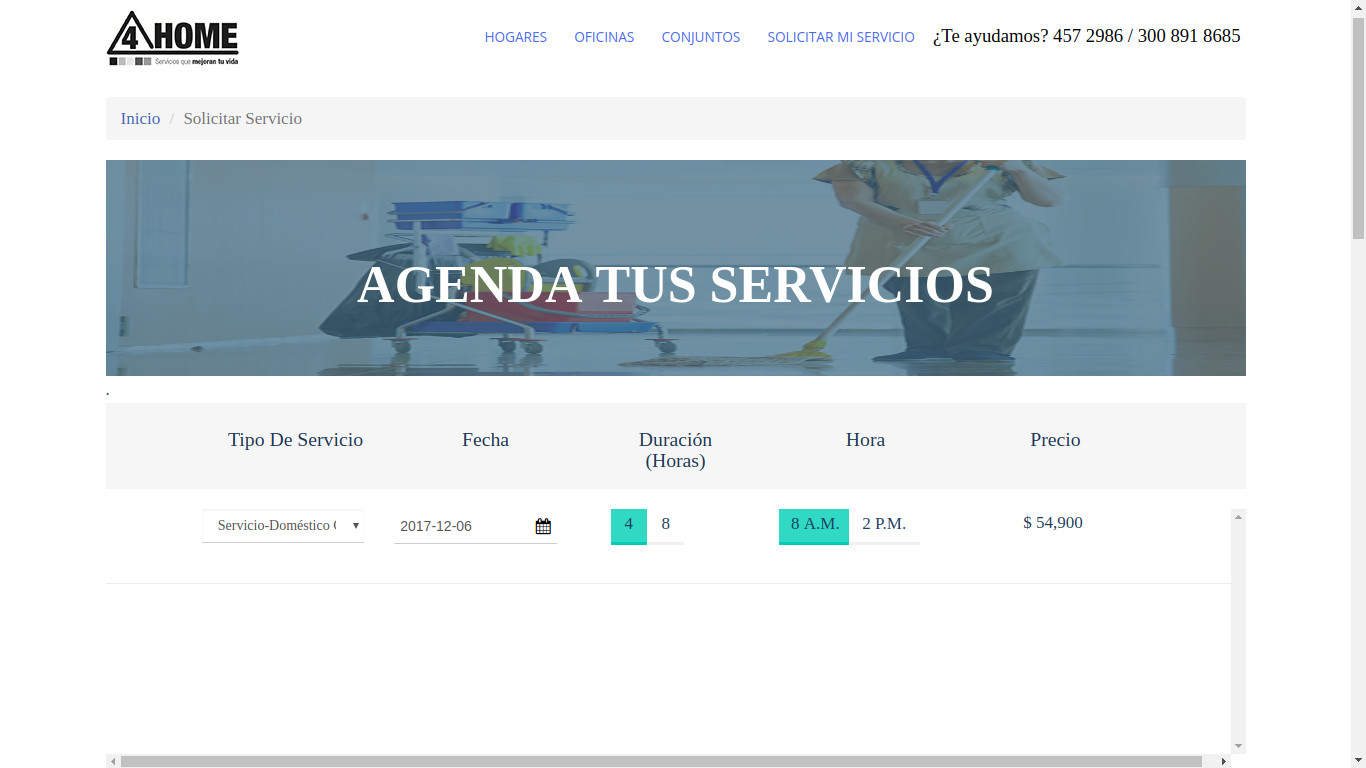
\includegraphics[width=.9\textwidth]{img/4home1.png}
\end{center}
\vspace{1cm}
\begin{center}
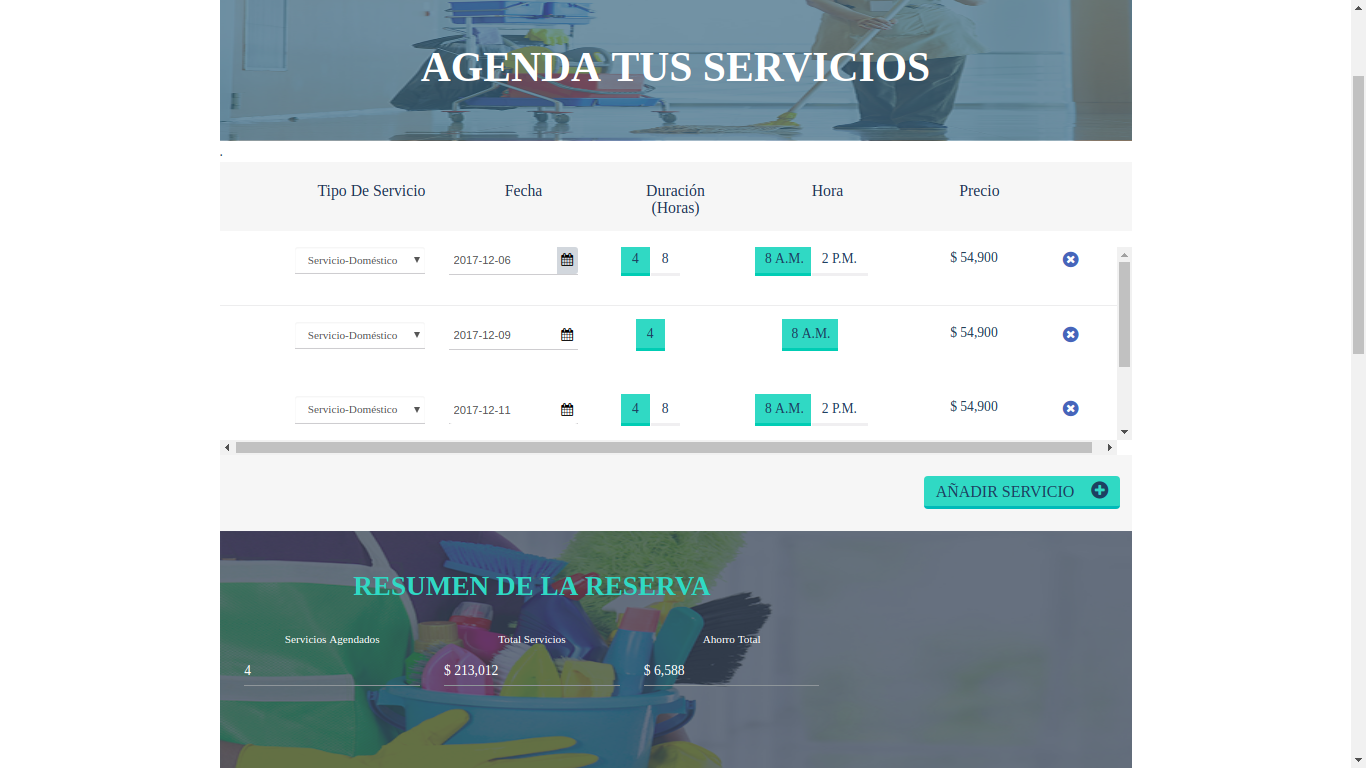
\includegraphics[width=.9\textwidth]{img/4home2.png}
\end{center}

\newpage
\makesidebarcommon % Print the sidebar
\begin{center}
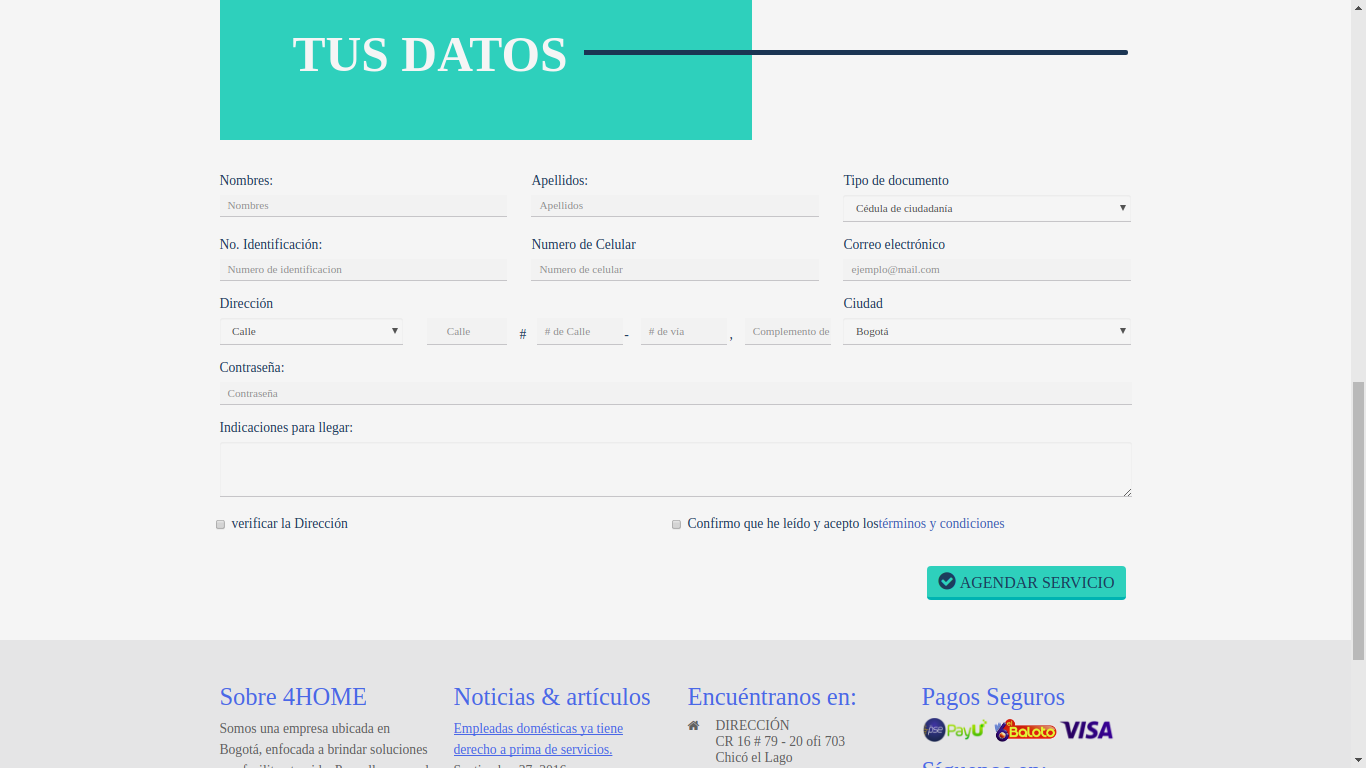
\includegraphics[width=.9\textwidth]{img/4home3.png} 
\end{center}


\newpage
\makesidebarcommon % Print the sidebar
\subsection{GanaGana App}
\begin{flushleft}
La aplicación cuenta con las siguientes características
\begin{itemize}
\item Un sistema de autenticación y almacenamiento de información en firebase
\item Primera interfaz de usuario con accesos rápidos, sidebar, slides publicitarios.
\end{itemize}
\end{flushleft}
\begin{center}
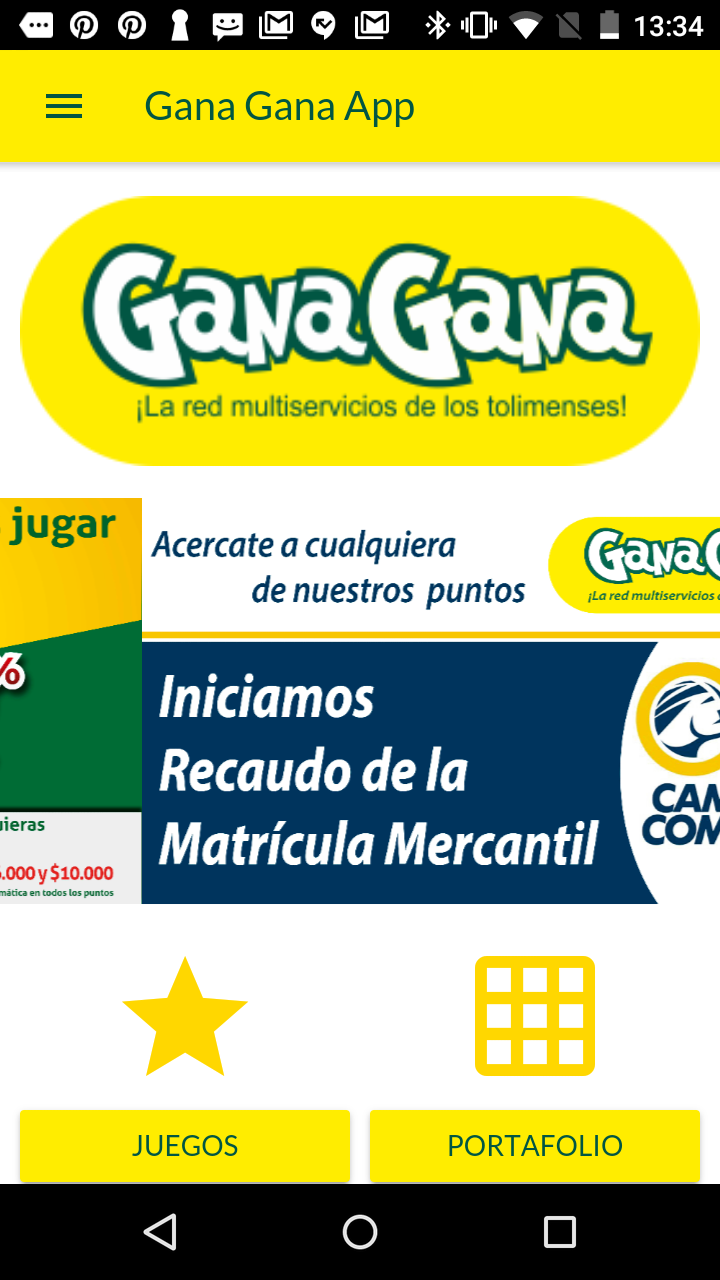
\includegraphics[width=.3\textwidth]{img/ganagana1.png}
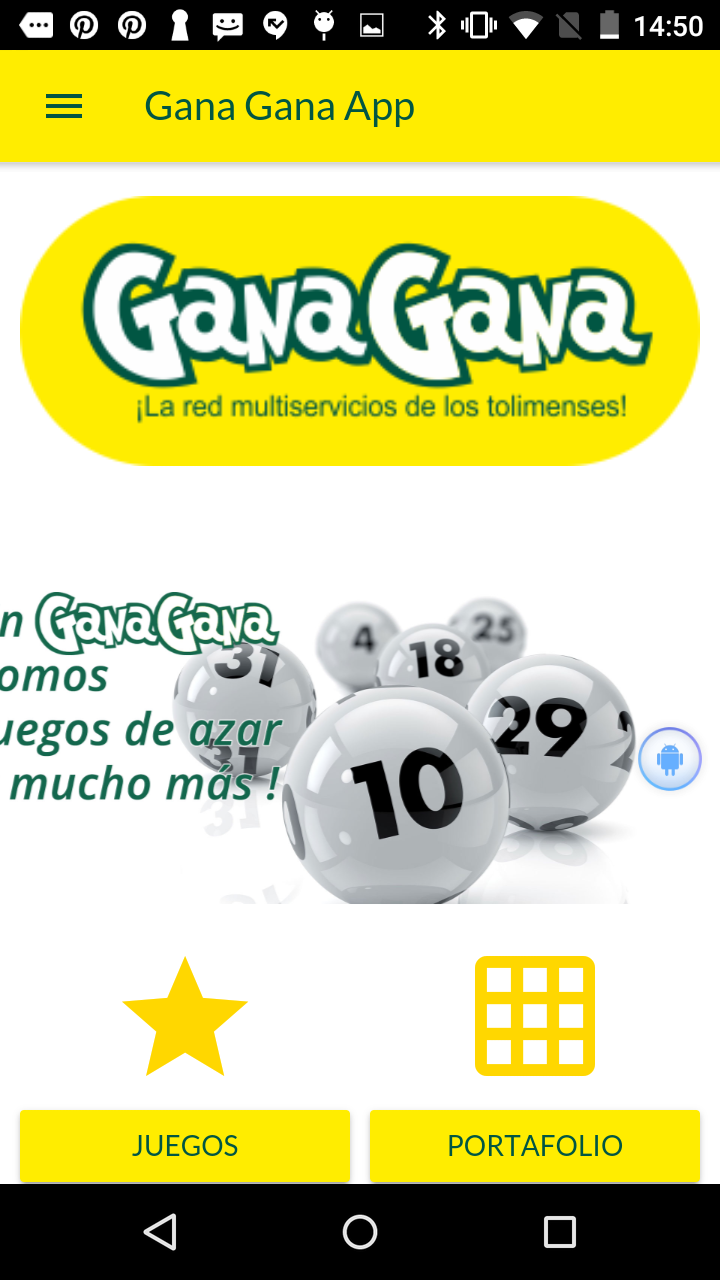
\includegraphics[width=.3\textwidth]{img/ganagana2.png}
\end{center}
\vspace{1cm}
\begin{itemize}
\item Juego de arma parejas para entretención y publicidad
\item Kit de la suerte que consistía en recorrer toda la ciudad en busca de códigos QR, esto a fin de premiar a quien consiguiera todos.
\end{itemize}
\begin{center}
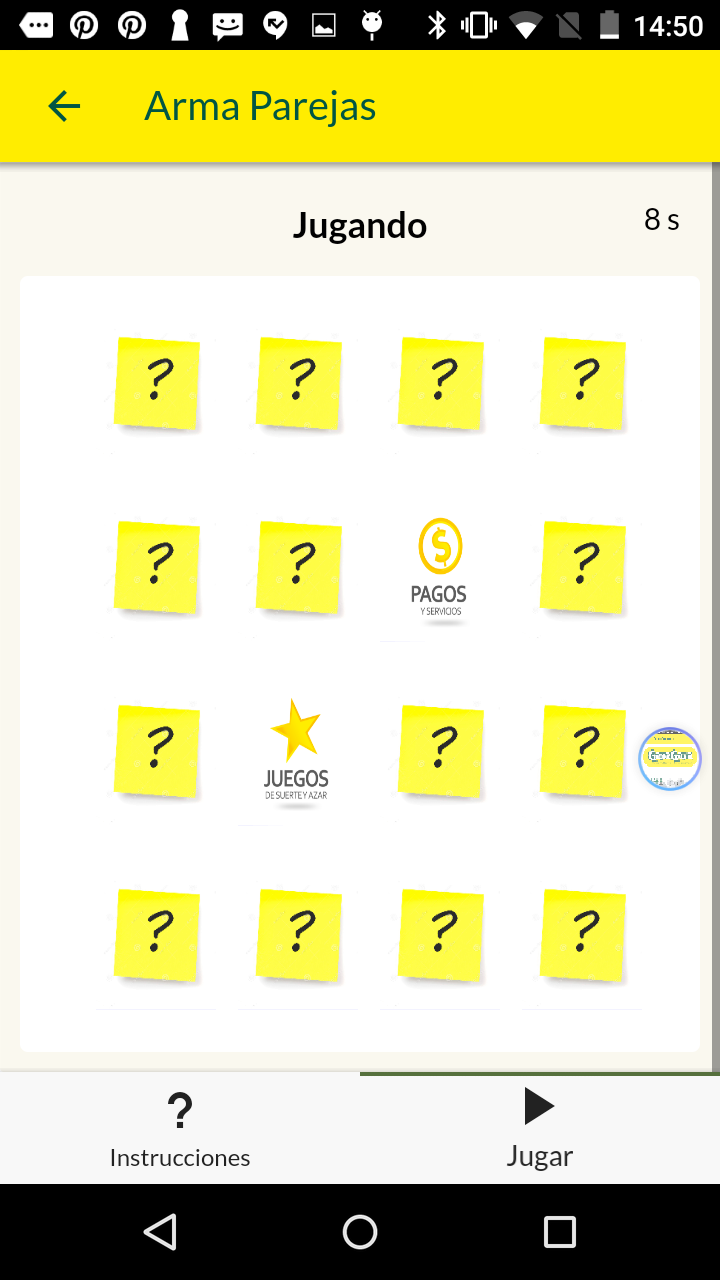
\includegraphics[width=.3\textwidth]{img/ganagana3.png} 
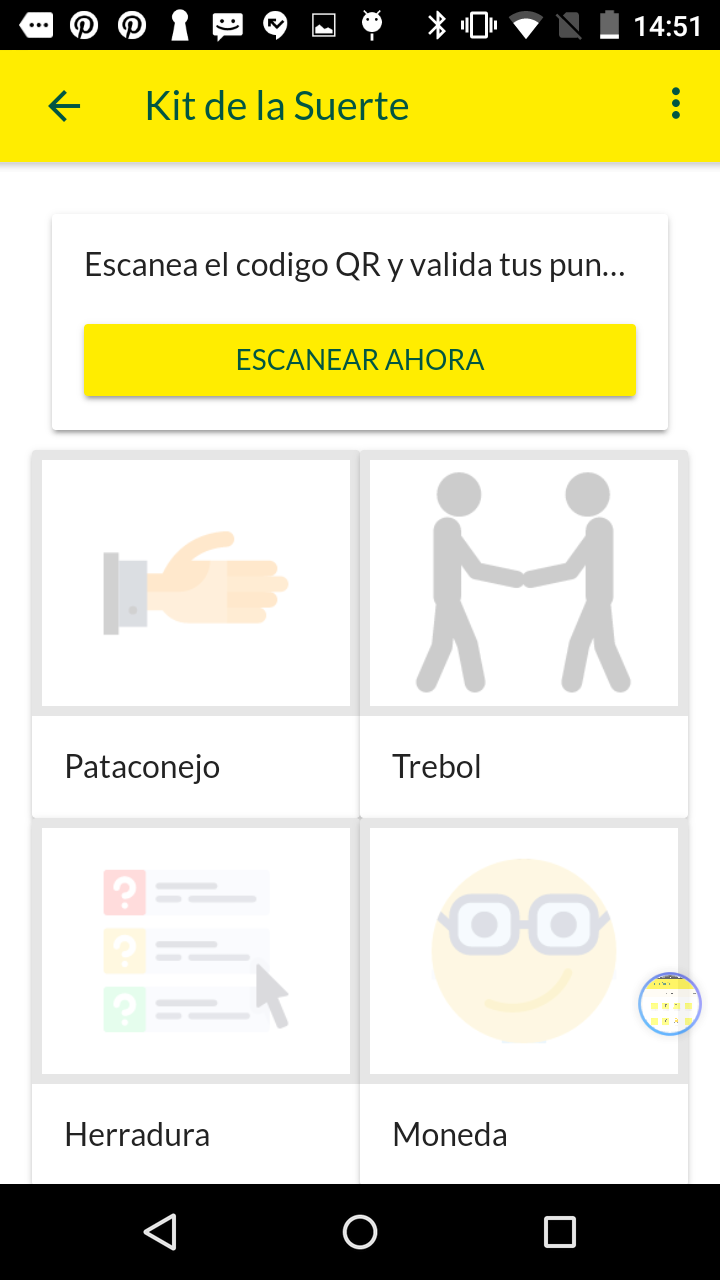
\includegraphics[width=.3\textwidth]{img/ganagana4.png} 
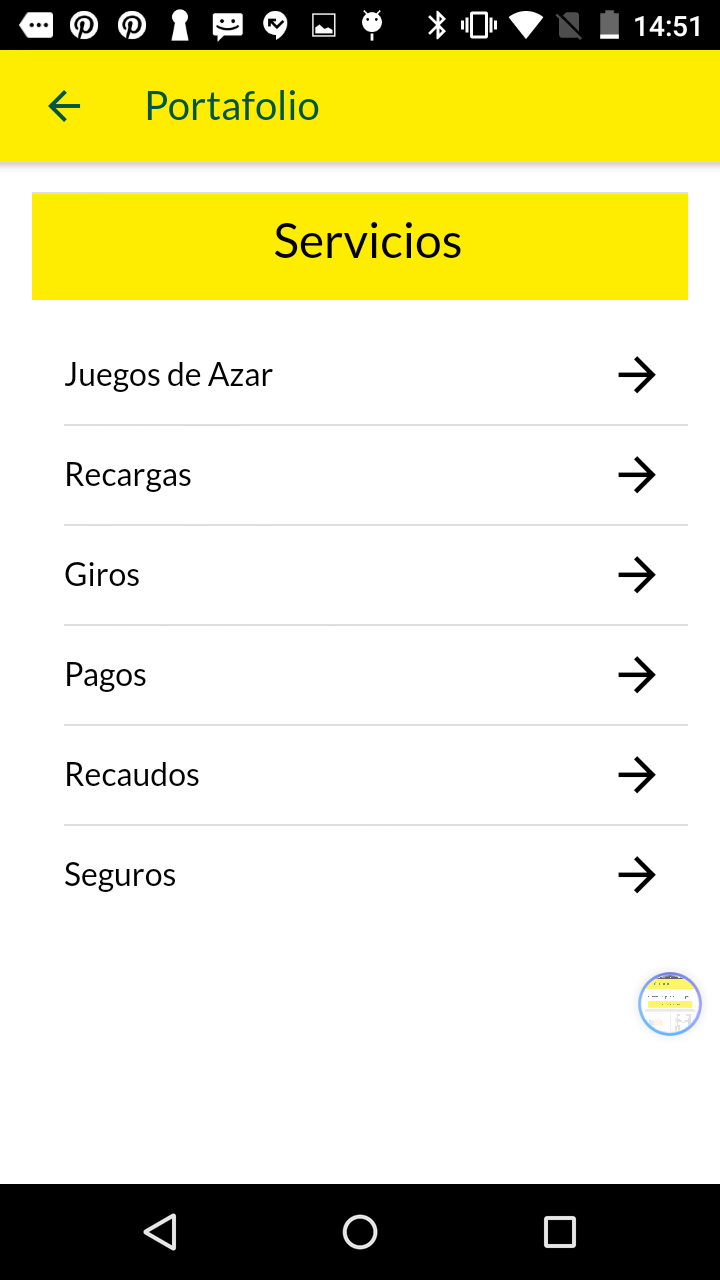
\includegraphics[width=.3\textwidth]{img/ganagana5.png} 
\end{center}
\newpage
\makesidebarcommon % Print the sidebar
\begin{itemize}
\item Portafolio de servicios que brinda la empresa.
\item Generador de numero de la suerte
\item Simulador de Giros
\end{itemize}
\begin{center}
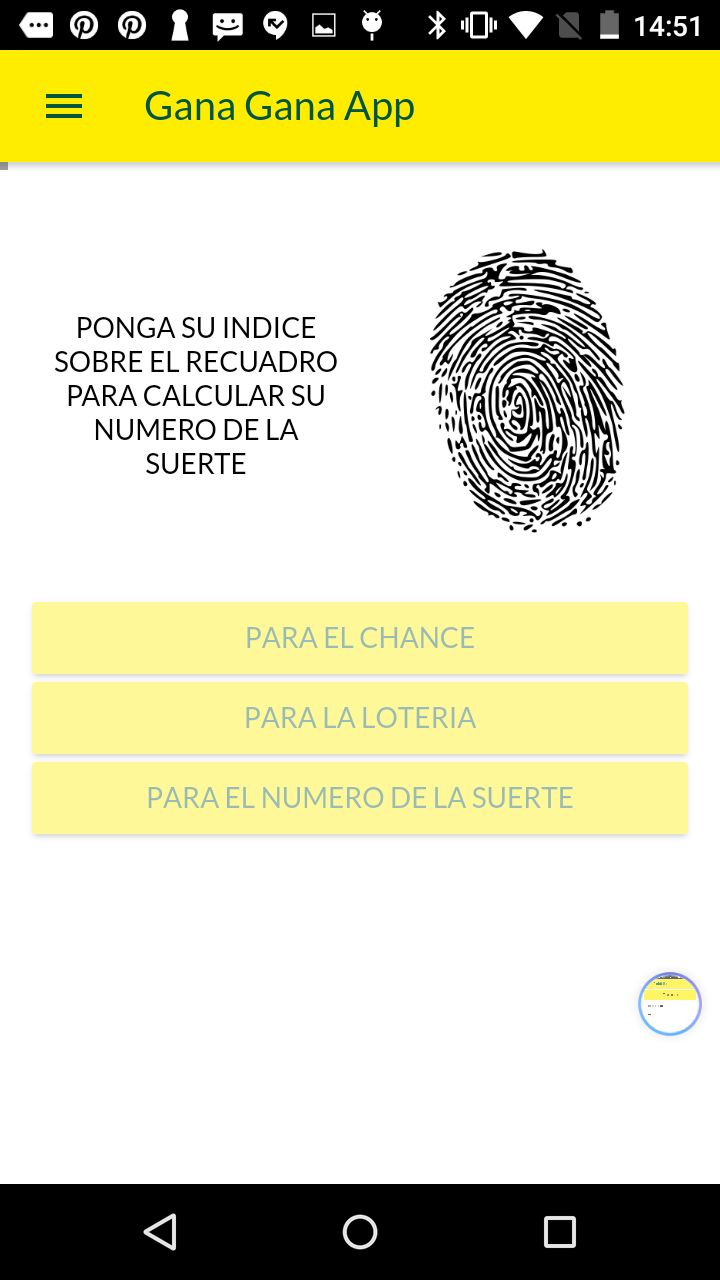
\includegraphics[width=.3\textwidth]{img/ganagana6.png} 
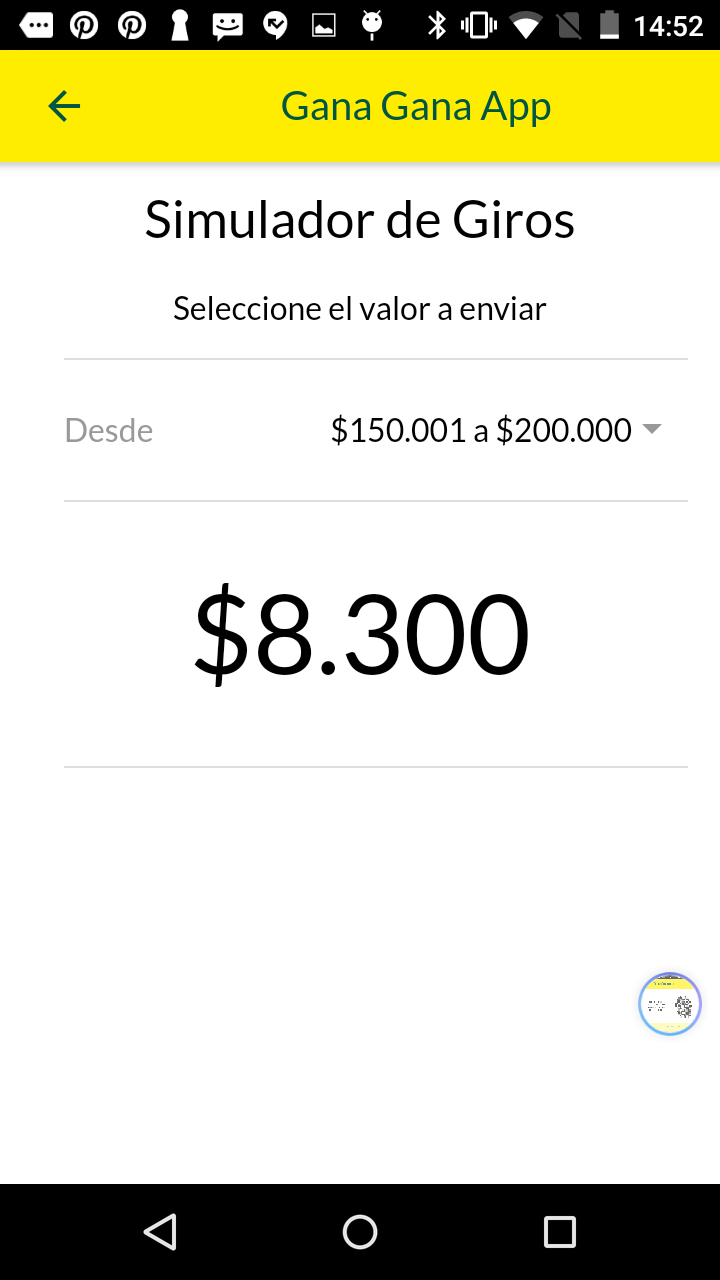
\includegraphics[width=.3\textwidth]{img/ganagana7.png} 
\end{center}
\end{document} 

